\section{Theory}

\subsection{Introduction}

Hall effect occurs when a current-carrying conductor is placed in a perpendicular magnetic field, causing charge carriers to experience the Lorentz force.
The force deflects the carriers to one side of the conductor, creating a transverse voltage, across the conductor, called the Hall voltage. The polarity of the voltage indicates the type of charge carriers (positive for holes and
negative for electrons). 
Magnetoresistance arises because the drift
velocities of charge carriers are not uniform. In the presence of an external magnetic field, the Hall voltage balances the Lorentz force for carriers with the mean velocity. Slower carriers are overcompensated, while faster ones are under compensated, leading to trajectories deviating from the applied field.
This reduces the mean free path, hence increasing resistivity.

\subsection{Theory}
Consider the Drude model of electrical conductivity. The average momentum of particles in presence of a magnetic field is,

\begin{align} \label{eq1}
    \frac{d\vect{p}}{dt} = -e\left(\vect{E}+\frac{\vect{p}}{m}\cross\vect{B}\right)-\frac{\vect{p}}{\tau}
\end{align}

where $\vect{p}$ is the average momentum of a particle with mass $m$ and mean time before consecutive collisions $\tau$. Here let's $\mu = \mu_0(1+\chi_m)\approx\mu_0$ for Bi (since $\chi_m \sim 10^{-4}$). Consider Fig. \ref{1} where $\vect{E}$ is applied from the $x$-direction and $\vect{H}$ is along $z$-axis. Since $\frac{d\vect{p}}{dt}=0$ at steady state, we can write from Eq. \label{eq1},

\begin{figure}
    \centering
    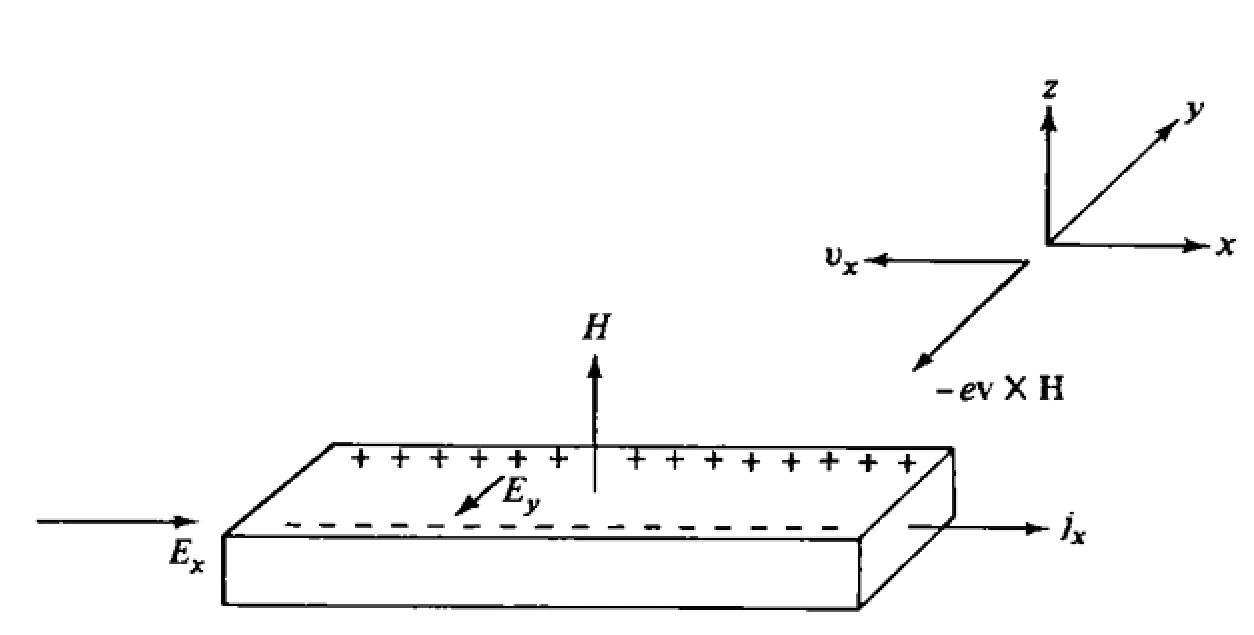
\includegraphics[width=1\columnwidth]{images/d.png}
    \caption{Schematic diagram showing the direction of the fields and current}
    \label{1}
\end{figure}

\begin{align}
    0 &= -eE_x - \omega_c p_y-\frac{p_x}{\tau}\\
    0 &= -eE_y + \omega_c p_x-\frac{p_y}{\tau}\\
    \text{where } \omega_c &= \frac{\mu_0eH}{m}\nonumber
\end{align}

Now we know $\vect{J}=\sigma\vect{E}$, where $\sigma$ is the conductivity from Drude model $=ne^2\tau/m$ and $\vect{J}$ is the current density. Hence we can write the above equations as,

\begin{figure*}
    \centering
    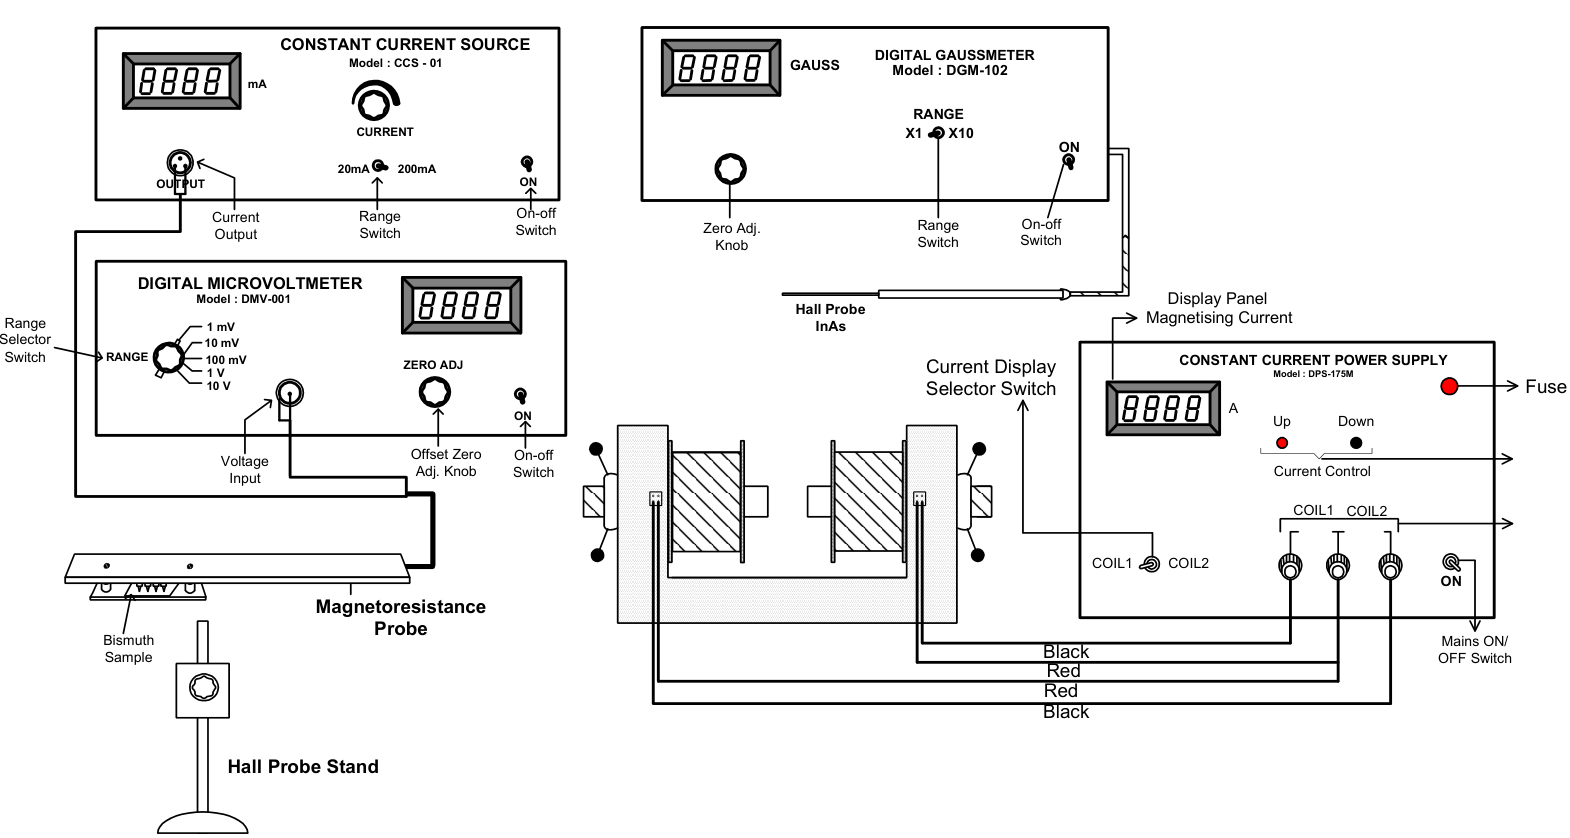
\includegraphics[width=1.7\columnwidth]{images/panel.png}
    \caption{Panel Diagram of the experimental setup}
    \label{expt}
\end{figure*}

\begin{align}
    \sigma E_x = \omega_c J_y\tau+J_x \label{eq4}\\
    \sigma E_y = -\omega_c J_x\tau+J_y \label{eq5}
\end{align}

When Lorentz force is balanced by the electrostatic force, $J_y=0$. Hence Eq. \ref{eq5} becomes,

\begin{align} \label{eq6}
    E_y = R_HBJ_y \text{, where }R_H = -\frac{1}{ne} 
\end{align}

Here, $R_H$ is called the Hall coefficient. Additionally, for a given magnetic field and input current, $V_H$ is inversely proportional to the carrier density $n$, which is linked to the material’s resistivity. The conductivity $\sigma$ of a material is given by $\sigma = ne\mu$, where $\mu$ is the carrier mobility. We can rewrite the above equation to use experimentally as,

\begin{align} \label{eq7}
    R_H = \frac{tV_H}{IB}
\end{align}

where $V_H$ is the Hall voltage, $t$ is the thickness of the sample, $I$ is the current and $H$ is the external magnetic field applied. Similarly from Eq. \ref{eq4}, we can get the magnetoresistance ($R_m$) as the ratio of the voltage $V$ and current $I$,

\begin{align} \label{eq8}
    R_m = \frac{V}{I}
\end{align}


Since Hall voltage is generally not a constant, but a function of the magnetic field, so will be the Hall coefficient.

Ordinary magnetoresistance can be classified into three distinct cases. In metals with closed Fermi surfaces, electrons are constrained to their orbits in k-space, and the magnetic field increases the cyclotron frequency of the electron in its closed orbit.
For metals with equal numbers of electrons and
holes, the magnetoresistance increases with $H$ up to the highest fields measured and is independent of crystallographic orientation, as seen in materials like bismuth. Metals containing Fermi surfaces with open orbits in certain crystallographic directions exhibit large magnetoresistance for fields applied in those directions, whereas resistance saturates in other directions where the orbits are closed.

Experimentally, $R$ provides a means to measure mobility of the charge carrier in a material. By the combination of Hall coefficient and resistivity measurements, information about carrier density, mobility, and impurity concentrations can be obtained. However, $R = 1/nq$ derived from Hall effect measurements may not always match directly measured values
due to the energy-dependent distribution of carriers, as
those with higher velocities experience greater deviations
in a magnetic field.

% =================================================
\section{Experimental Setup}
Fig. \ref{expt} shows the experimental setup for observing Hall effect. A detailed list of all the apparatus required is listed below.

Experimental procedure is briefed below in the next section.

\subsection*{Apparatus}

\begin{enumerate}
    \item Magnetoresistance and Hall probes
    \item Samples of Bismuth ($t = 0.5$ mm)
    \item Hall Effect Set-up (DHE-22)
    \item Electromagnet (EMU-75V)
    \item Constant Current Source (CCS-01)
    \item Constant Current Power Supply (DPS-175)
    \item Digital Gaussmeter (DGM-102)
    \item Digital Microvoltmeter (DMV-001)
\end{enumerate}
